\documentclass[10pt,letterpaper]{article} 
\usepackage{tikz}
\usepackage{tools}
\usepackage{enumitem,caption}
\usepackage{listings}
\usepackage{xepersian}
\lstset{language=Python}
%\lstset{frame=lines}
%\lstset{caption={Insert code directly in your document}}
\lstset{label={lst:code_direct}}
\lstset{basicstyle=\footnotesize}

%\usepackage{graphicx}‎‎
%\usefonttheme{serif}‎
%\usepackage{ptext}‎
%\usepackage{xepersian}
%\settextfont{B Nazanin}
\usepackage{lipsum}
\setlength{\parindent}{0pt}
\newcommand{\pf}{$\blacksquare$}

\newcommand{\Span}{\text{Span}}
\newcommand{\NF}{\text{NF}}
\newcommand{\EDFA}{\text{EDFA}}
\newcommand{\ASE}{\text{ASE}}

\newcommand{\bns}{\textit{broadcast-and-select}  architecture}
\newcommand{\Bns}{\textit{Broadcast-and-select} architecture}

\newcommand{\rns}{\textit{route-and-select} architecture}
\newcommand{\Rns}{\textit{Route-and-select} architecture}

\newcounter{QuestionNumber}
\setcounter{QuestionNumber}{1}

\newcommand{\temp}{{\color{red}{temp}}}

\newcommand{\Q}{
\textbf{سوال \theQuestionNumber)}
\stepcounter{QuestionNumber}
}
\newcommand{\EX}{\Bbb E}
\newcommand{\nl}{\newline\newline}
\begin{document}
\large
\begin{center}
به نام او

پایان ترم شبکه های مخابرات نوری

مدت زمان: 120 دقیقه
\hl
\end{center}

\Q

در توپولوژی مشبک زیر، فرض کنید طول هر لینک 1000 کیلومتر و سرعت انتشار نور در فیبر 
$
2\times 10^8
$
متر بر ثانیه باشد. یک درخواست اتصال بین نودهای \lr{A} و \lr{D}، به نود \lr{A} می‌رسد. نود \lr{A} از \lr{PCE} (نود \lr{G}) درخواست محاسبه مسیر انجام می‌دهد و پس از دریافت پاسخ، دستور تنظیم سوئیچ را به نودهای کوتاهترین مسیر بین خود و نود \lr{D} (از جمله نود \lr{D}) ارسال می‌کند. هر نود پس از دریافت دستور تنظیم سوئیچ، در 10 میلی ثانیه اقدام به تنظیم سوئیچ خود کرده و دستور تنظیم سوئیج را به نود بعدی فوروارد می‌کند.

\begin{enumerate}[label=\alph*-]
\item
با فرض آن که هر نود پس از تنظیم سوئیچ خود، یک پیام تأیید به سمت نود A بفرستد، پس از چه مدت زمانی از رسیدن درخواست اتصال به نود A از لایه‌ی بالاتر، نود A می‌تواند ارسال را شروع کند؟ پاسخ را در هر دو حالت pipelined و غیر pipelined به دست آورید.
\item
اگر زمان تنظیم سوئیچ نود C برابر 
$
d_\text{C}
$
 باشد، نمودار مدت زمانی که طول می‌کشد تا نود A ارسال را شروع کند، بر حسب 
$
d_\text{C}
$
رسم کنید. فرض کنید ارسال به صورت pipelined باشد و هر نود پس از تنظیم سوئیچ خود، یک پیام تأیید به سمت نود A می‌فرستد.
\end{enumerate}

(دقت کنید که نود A تنها زمانی اقدام به ارسال می‌کند که تأیید تنظیم سوئیچ را از تمام نودهای مسیر دریافت کرده باشد.)

\begin{figure}[h]
\centering
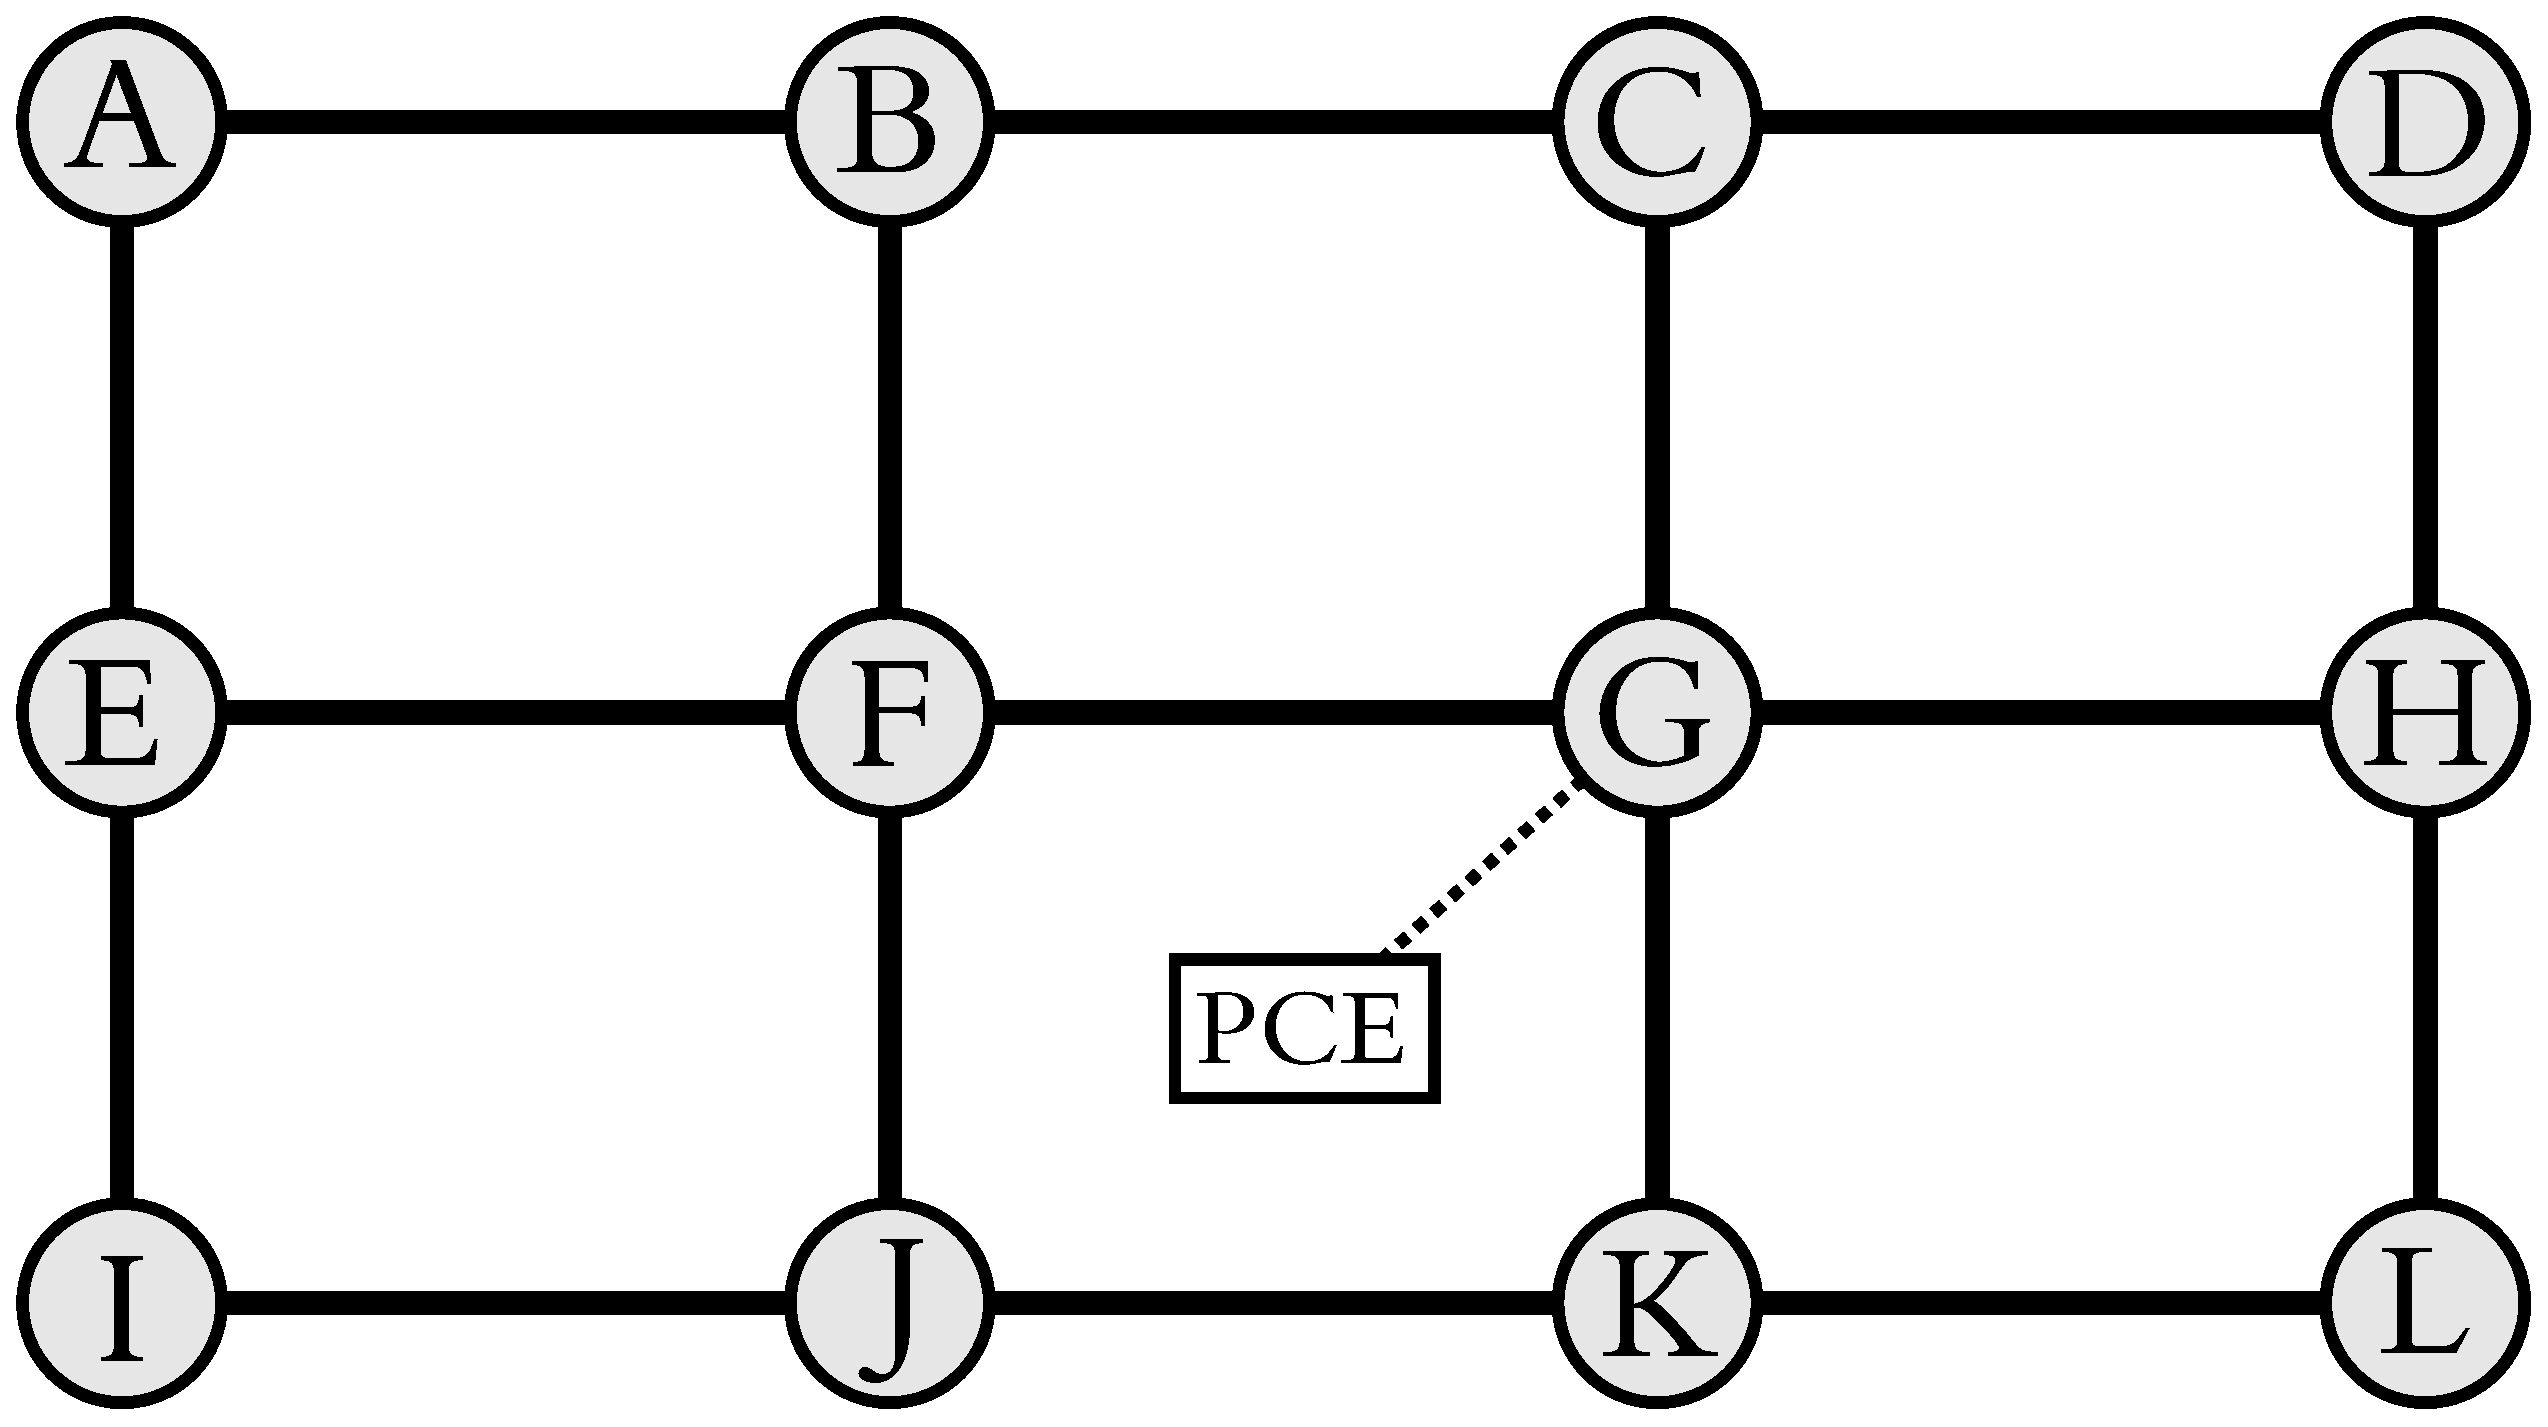
\includegraphics[width=80mm]{dynamic_final.eps}
\end{figure}

\newpage

\Q

شبکه‌ی نوری زیر مفروض است. 6 اتصال بین نودهای شبکه در جدول 1 داده شده است که هر اتصال، دارای حفاظت $1+1$ می‌باشد. دقت کنید که در هر جهت ارسال روی لینک، فیبر مجزا موجود است. تخصیص طول موج را به 6 اتصال داده شده با استفاده از الگوریتم ابتکاری first-fit اعمال کنید.

\begin{figure}[h]
\centering
\includegraphics[width=70mm]{protection_final.eps}
\end{figure}

\begin{table}[h]
\Large
\centering
\begin{tabular}{|c|c|c|}
\hline
شماره‌ی اتصال&مسیر اصلی&مسیر حفاظت
\\\hline
1&$\text{A}\to\text{B}\to\text{D}$&$\text{A}\to\text{E}\to\text{D}$
\\\hline
2&$\text{F}\to\text{D}\to\text{B}$&$\text{F}\to\text{E}\to\text{A}\to\text{B}$
\\\hline
3&$\text{A}\to\text{E}\to\text{F}$&$\text{A}\to\text{B}\to\text{C}\to\text{F}$
\\\hline
4&$\text{B}\to\text{D}\to\text{F}$&$\text{B}\to\text{C}\to\text{F}$
\\\hline
5&$\text{B}\to\text{A}\to\text{E}$&$\text{B}\to\text{C}\to\text{D}\to\text{E}$
\\\hline
6&$\text{E}\to\text{D}\to\text{C}$&$\text{E}\to\text{F}\to\text{C}$
\\\hline
\end{tabular}
\caption{}
\end{table}

\newpage

\Q

در شبکه‌ی زیر، اگر \lr{optical reach} برابر 1000 کیلومتر باشد، جزایر شفافیت (\lr{Islands of Transparency}) را به گونه‌ای مشخص کنید که در هر جزیره، اتصال تمام-نوری (\lr{All-Optical}) بین هر دو نود درون جزیره وجود داشته باشد.

\begin{figure}[h]
\centering
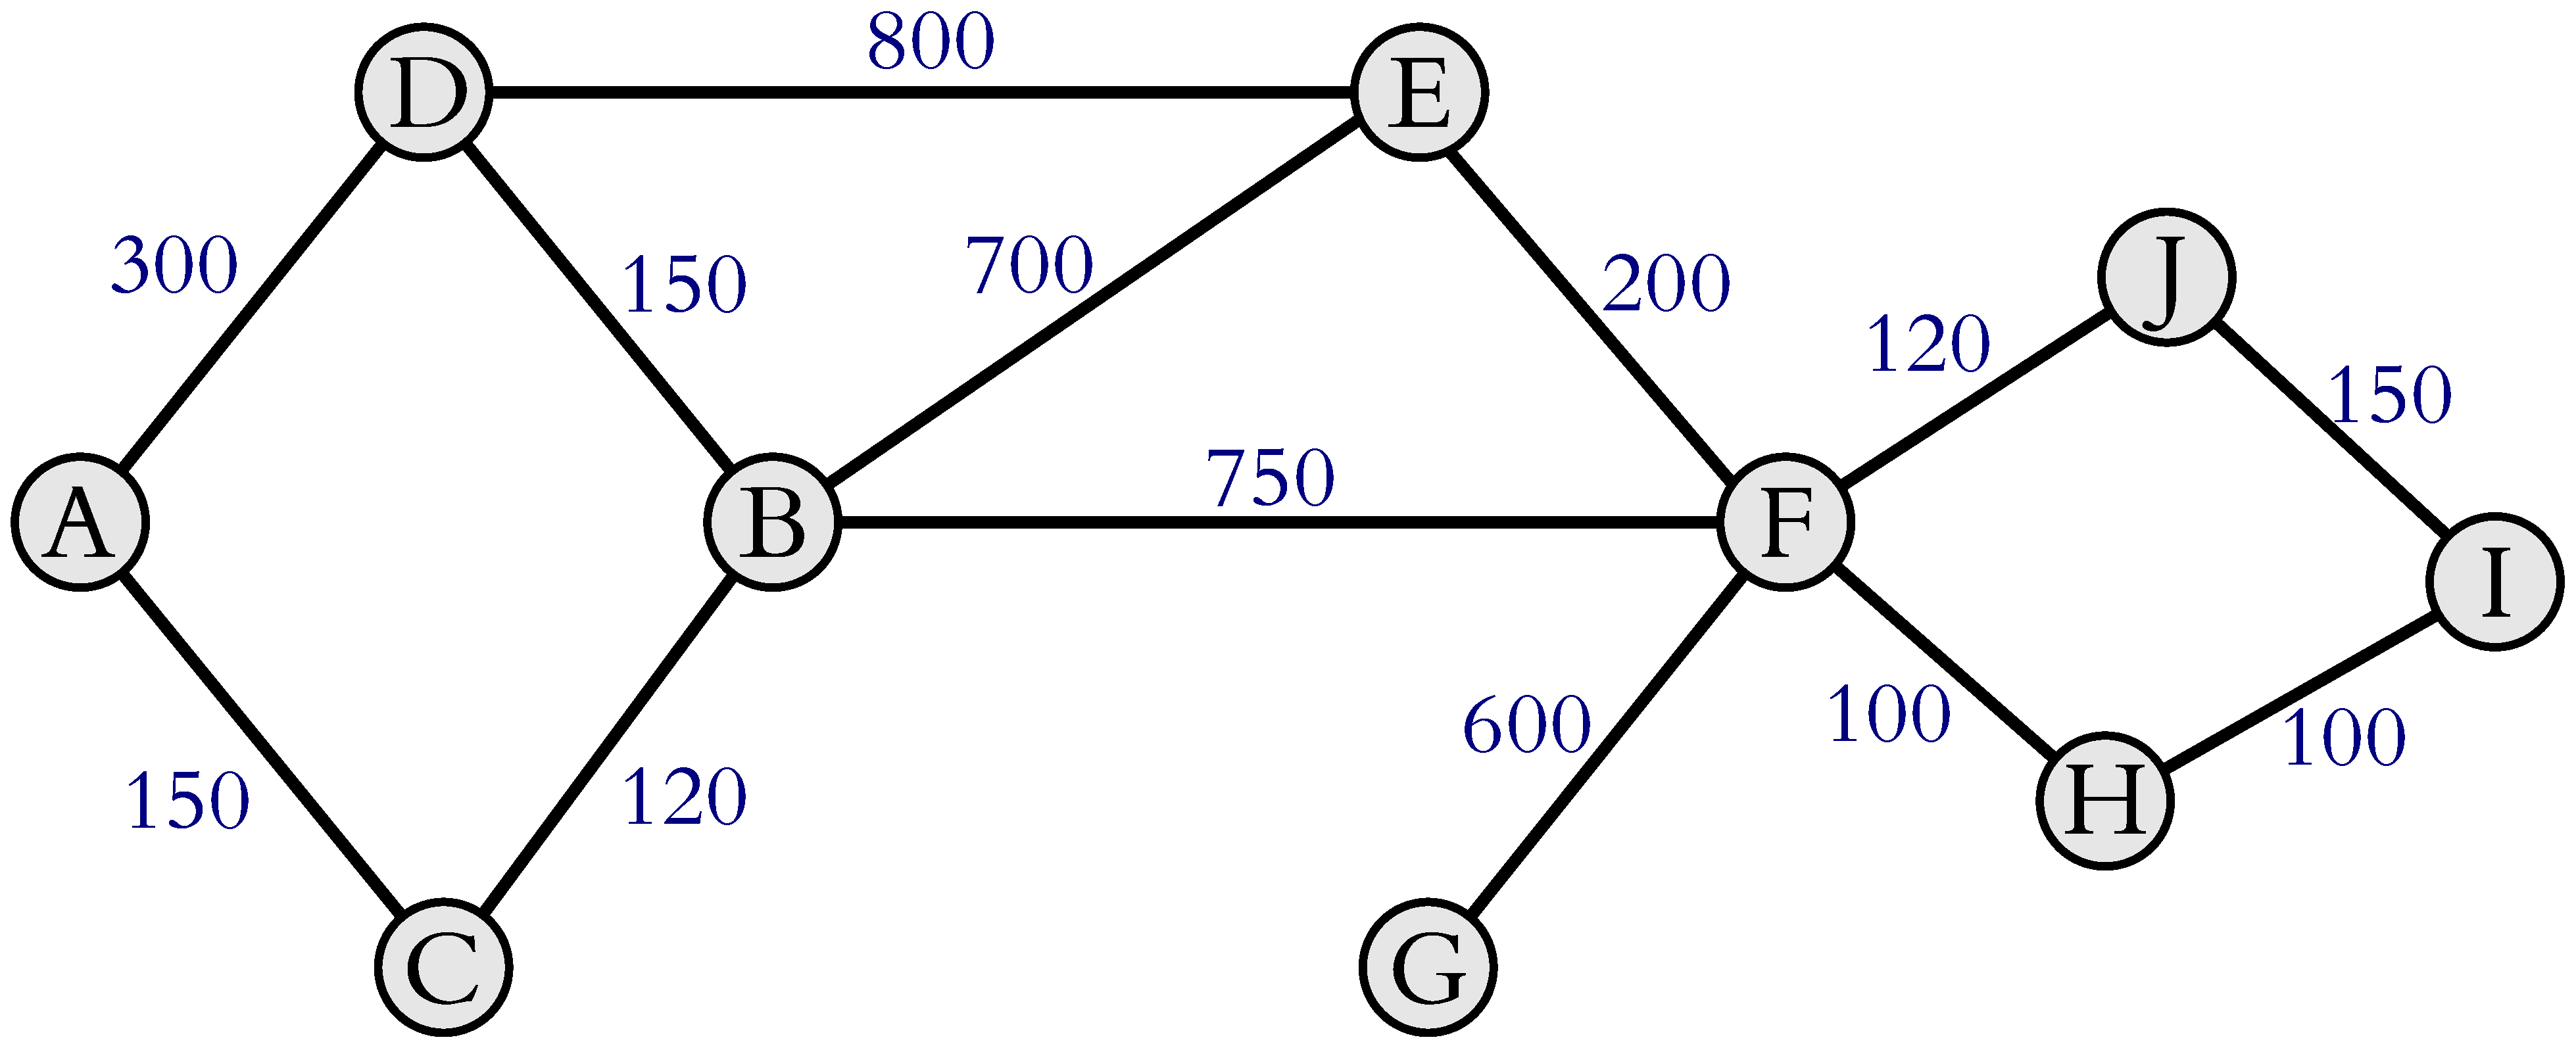
\includegraphics[width=120mm]{Islands_of_Transparency_Final.eps}
\end{figure}

\newpage

\Q

در شبکه‌ی شکل زیر، 4 اتصال دو طرفه بین نودهای مختلف به همراه مشخصات این اتصال‌ها در جدول 2 داده شده است. پهنای باند هر طول موج برابر
40GHz
بوده، ارسال با شکل پالس sinc انجام می‌شود و فرض کنید دو طول موج 
$
\lambda_1
$
و
$
\lambda_2
$
روی هر فیبر موجود است. همچنین، طول موج اختصاص داده شده به هر دو جهت یک اتصال یکسان است.

\begin{enumerate}[label=\alph*-]
\item
بدون استفاده از گرومینگ، تخصیص طول موج را برای اتصال های داده شده به کمک first-fit انجام دهید. آیا اتصال بلاک شده‌ای خواهیم داشت؟
\item
اگر از گرومینگ میانی برای تجمیع نرخ ها استفاده کنیم، در کدام یک از نودها باید گرومینگ انجام شود؟ مشخص کنید در نودهایی که گرومینگ اجرا می‌شود، کدام درخواست ها تجمیع می‌شوند. آیا اتصال بلاک شده‌ای خواهیم داشت؟
\end{enumerate}

\begin{figure}[h]
\centering
\includegraphics[width=70mm]{grooming_final.eps}
\end{figure}

\begin{table}[h]
\Large
\centering
\begin{tabular}{|c|c|c|}
\hline
شماره اتصال&نرخ بیت درخواستی&نوع مدولاسیون
\\\hline
1&$2.5\text{Gbps}$&PM-16QAM
\\\hline
2&4Gbps&PM-QPSK
\\\hline
3&$2.5\text{Gbps}$&PM-16QAM
\\\hline
4&$2.5\text{Gbps}$&PM-QPSK
\\\hline
\end{tabular}
\caption{}
\end{table}

%\begin{table}[h]
%\Large
%\centering
%\begin{tabular}{|c|c|c|c|c|}
%\hline
%شماره اتصال&نود مبدأ&نود مقصد&نرخ بیت درخواستی&نوع مدولاسیون
%\\\hline
%1&K&B&$2.5\text{Gbps}$&PM-16QAM
%\\\hline
%2&G&D&4Gbps&PM-QPSK
%\\\hline
%3&C&E&$2.5\text{Gbps}$&PM-16QAM
%\\\hline
%4&H&D&$2.5\text{Gbps}$&PM-QPSK
%\\\hline
%\end{tabular}
%\caption{}
%\end{table}

\end{document}